% =============================================================================
%  PATENT APPLICATION
%  SYSTEM AND METHOD FOR CONFLICT-FREE FLIGHT PLAN SCHEDULING
%  IN URBAN AIR MOBILITY NETWORKS
% =============================================================================

\documentclass[12pt,a4paper]{article}

% ---------- Packages ----------
\usepackage[utf8]{inputenc}
\usepackage[T1]{fontenc}
\usepackage[english]{babel}
\usepackage{geometry}
\usepackage{amsmath,amssymb,amsthm}
\usepackage{algorithm}
\usepackage{algpseudocode}
\usepackage{array}
\usepackage{booktabs}
\usepackage{enumitem}
\usepackage{titlesec}
\usepackage{fancyhdr}
\usepackage{graphicx}
\usepackage{xcolor}
\usepackage{hyperref}
\usepackage{tikz}
\usetikzlibrary{arrows.meta, positioning, shapes.geometric, fit, calc}

\geometry{
  top=2.5cm, bottom=2.5cm,
  left=3cm, right=2.5cm
}

% ---------- Header / Footer ----------
\pagestyle{fancy}
\fancyhf{}
\fancyhead[L]{\small PATENT APPLICATION}
\fancyhead[R]{\small CONFLICT-FREE UAM FLIGHT SCHEDULING}
\fancyfoot[C]{\thepage}
\renewcommand{\headrulewidth}{0.4pt}

% ---------- Section formatting ----------
\titleformat{\section}[block]
  {\normalfont\large\bfseries\centering}
  {}
  {0pt}
  {\MakeUppercase}

\titleformat{\subsection}[runin]
  {\normalfont\bfseries}
  {}
  {0pt}
  {}[.\quad]

% ---------- Theorem environments ----------
\newtheorem{theorem}{Theorem}
\newtheorem{lemma}[theorem]{Lemma}
\newtheorem{proposition}[theorem]{Proposition}
\newtheorem{definition}{Definition}
\newtheorem{claim}{Claim}

% ---------- Convenience macros ----------
\newcommand{\MSD}{\mathrm{MSD}}
\newcommand{\hmin}{h_{\min}}
\newcommand{\tdep}{t_{\mathrm{dep}}}
\newcommand{\twpN}{t_{\mathrm{wpN}}}
\newcommand{\ttouch}{t_{\mathrm{touch}}}
\newcommand{\tto}{t_{\mathrm{takeoff}}}
\newcommand{\tland}{t_{\mathrm{land}}}
\newcommand{\lane}{\tau_{\mathrm{lane}}}

% =============================================================================
\begin{document}
% =============================================================================

% ---------- Title page ----------
\begin{center}
  \vspace*{1.5cm}
  {\LARGE\bfseries PATENT APPLICATION}\\[0.6cm]
  {\large Application Number: \underline{\hspace{4cm}}}\\[0.2cm]
  {\large Filing Date: \underline{\hspace{4cm}}}\\[1.5cm]

  \rule{\linewidth}{1pt}\\[0.4cm]
  {\LARGE\bfseries
    SYSTEM AND METHOD FOR CONFLICT-FREE FLIGHT PLAN\\
    SCHEDULING IN URBAN AIR MOBILITY NETWORKS\\
    USING MONOTONE FIXED-POINT CONSTRAINT RESOLUTION
  }\\[0.4cm]
  \rule{\linewidth}{1pt}\\[1.5cm]

  \begin{tabular}{ll}
    \textbf{Inventors:}  & \underline{\hspace{8cm}} \\[0.3cm]
    \textbf{Assignee:}   & \underline{\hspace{8cm}} \\[0.3cm]
    \textbf{IPC Class:}  & G08G~5/00;\; G08G~5/04;\; G01C~21/20;\; G06F~17/11 \\[0.3cm]
    \textbf{Priority:}   & \underline{\hspace{8cm}} \\
  \end{tabular}
\end{center}

\newpage
\tableofcontents
\newpage

% =============================================================================
\section{Abstract}
% =============================================================================

A system and method are disclosed for resolving scheduling conflicts among
Urban Air Mobility (UAM) flight plans in a shared multi-vertiport airspace
network.  A new flight-plan request is evaluated against an existing set of
approved plans by enforcing four physical safety constraints: (C1)~minimum
spatial separation between drones sharing the same horizontal lane segment;
(C2)~mutual exclusion of the vertical takeoff corridor above the departure
vertiport; (C3)~mutual exclusion of the vertical landing corridor above the
destination vertiport; and (C4)~pad-occupancy exclusion at the landing pad.

Each constraint is formulated as a monotone, non-decreasing function that maps
a candidate departure delay to a feasible departure delay.  Because the
composition of monotone bounded functions is itself monotone and bounded, the
Knaster--Tarski fixed-point theorem guarantees that iterating the constraint
pipeline~(C1\,$\to$\,C2\,$\to$\,C3\,$\to$\,C4) converges to the
\emph{minimum feasible delay} in a finite number of steps.  The request is
approved if and only if this minimum delay does not exceed a caller-specified
maximum wait tolerance.  A priority-based sequential resolution strategy is
additionally disclosed for handling batches of simultaneous requests without
post-approval conflicts.

% =============================================================================
\section{Field of the Invention}
% =============================================================================

The present invention relates to air traffic management, and more particularly
to automated conflict detection and resolution for small unmanned aircraft
systems (UAS) and electric vertical take-off and landing (eVTOL) vehicles
operating within urban air mobility (UAM) networks comprising multiple
vertiports.

% =============================================================================
\section{Background of the Invention}
% =============================================================================

Urban air mobility networks employ large fleets of autonomous or
semi-autonomous aerial vehicles that depart from and arrive at vertiports
equipped with a finite number of landing pads.  Safe and efficient operation
requires that no two vehicles simultaneously occupy the same spatial region.
Conflicts may arise in at least four distinct spatial zones:

\begin{enumerate}[label=(\arabic*)]
  \item \textbf{Horizontal lane segments.}  Vehicles sharing a waypoint-to-waypoint
    lane must maintain a minimum spatial separation to prevent mid-air collision,
    accounting for differing speeds.

  \item \textbf{Vertical takeoff corridor.}  The confined airspace immediately
    above a vertiport allows only one vehicle to ascend at any given time.

  \item \textbf{Vertical landing corridor.}  Similarly, the confined approach
    airspace above a destination vertiport permits only one vehicle to descend
    at any given time.  Importantly, the takeoff and landing corridors of any
    vertiport share the same physical volume, so ascent and descent operations
    at the same vertiport are mutually exclusive.

  \item \textbf{Landing pad surface.}  After touchdown, a vehicle occupies a
    pad for a finite service duration, preventing another vehicle from landing
    on the same pad.
\end{enumerate}

Prior art approaches typically address these conflicts by solving large mixed-
integer programs or by applying separated heuristics for each constraint
category.  Such methods are computationally expensive, may not guarantee a
global minimum delay, and do not provide formal convergence proofs suitable for
safety-critical aviation applications.  There exists a need for a lightweight,
formally convergent conflict-resolution algorithm that can be deployed
on-board or in edge computing nodes of a UAM network manager.

% =============================================================================
\section{Summary of the Invention}
% =============================================================================

In one aspect, the invention provides a computer-implemented method for
conflict-free flight-plan scheduling comprising:

\begin{enumerate}[label=(\alph*)]
  \item Receiving a flight-plan request specifying a departure vertiport, a
    destination vertiport, an ordered sequence of waypoints, per-segment
    cruise speeds, vertical phase durations, a desired departure time, and a
    maximum tolerated wait time.

  \item Computing, for each of the four physical safety constraints (C1--C4),
    a monotone non-decreasing function $f_k\colon \mathbb{R}_{\ge 0} \to
    \mathbb{R}_{\ge 0}$ that maps a current delay to a delay sufficient to
    satisfy constraint $C_k$.

  \item Iterating the composed function $F = f_4 \circ f_3 \circ f_2 \circ f_1$
    from an initial delay of zero until the delay value converges within a
    numerical tolerance $\varepsilon$.

  \item Approving the flight plan with the converged delay if that delay does
    not exceed the maximum wait time; otherwise, rejecting the request with a
    structured explanation.

  \item When processing a batch of simultaneous requests, sorting requests by
    ascending priority and resolving them sequentially, augmenting the approved-
    plan pool after each approval.
\end{enumerate}

In another aspect, the invention provides a system comprising one or more
processors and non-transitory computer-readable media embodying instructions
that, when executed, perform the above method.

% =============================================================================
\section{Brief Description of the Drawings}
% =============================================================================

\begin{itemize}
  \item[\textbf{FIG.\,1}] is a schematic of the four conflict zones (C1--C4)
    along a UAM flight timeline.

  \item[\textbf{FIG.\,2}] is a graph showing the evolution of inter-drone
    distance along a shared lane segment, illustrating the derivation of the
    minimum headway $\hmin$.

  \item[\textbf{FIG.\,3}] is a flowchart of the fixed-point iteration algorithm
    for a single request.

  \item[\textbf{FIG.\,4}] is a timing diagram of the three-round cascade
    convergence example described herein.

  \item[\textbf{FIG.\,5}] is a flowchart of the priority-based batch resolution
    procedure.
\end{itemize}

% =============================================================================
\section{Detailed Description of Preferred Embodiments}
% =============================================================================

The following description sets forth specific details of embodiments of the
invention.  Like reference numerals denote like elements throughout the figures.

\subsection*{6.1\quad Network and Flight-Plan Model}

\paragraph{Vertiports and pads.}
A UAM network $\mathcal{V}$ consists of a finite set of vertiports
$\{V_1, V_2, \ldots\}$.  Each vertiport $V$ comprises one or more landing
pads $\{p_1, p_2, \ldots\}$.  Each pad $p$ has a service (occupation) duration
$\delta_p > 0$ seconds during which the pad is unavailable to other vehicles
after a touchdown event.

\paragraph{Flight plan.}
A flight plan $\Pi$ is a tuple
\[
  \Pi = \bigl(\,A,\, B,\, [w_0, w_1, \ldots, w_n],\, [v_0, \ldots, v_{n-1}],\,
             \tto,\, \tland,\, t_s,\, \text{pad}\bigr),
\]
where $A$ and $B$ are the departure and destination vertiports; $w_0, \ldots,
w_n$ are waypoints on horizontal lanes (vertiport positions are \emph{not}
included in this list); $v_k$ is the cruise speed on segment $k$ (i.e., from
$w_{k-1}$ to $w_k$ for $k=1,\ldots,n$, with $w_0$ the first airway entry
point and $w_n$ the last); $\tto$ and $\tland$ are the durations of the
vertical ascent and descent phases respectively; $t_s$ is the scheduled
departure time; and $\mathrm{pad}$ is the assigned landing pad (relevant for
approved plans).

\paragraph{Flight timeline.}
For a flight plan with departure time $t_s$ the key instants are:
\begin{align}
  \lane &= \sum_{k=1}^{n} \frac{\|w_k - w_{k-1}\|}{v_{k-1}},
  \label{eq:lane_time}\\
  \twpN &= t_s + \tto + \lane,
  \label{eq:twpn}\\
  \ttouch &= \twpN + \tland.
  \label{eq:ttouch}
\end{align}
The three phases partition the flight into: (i)~a vertical ascent of duration
$\tto$; (ii)~a horizontal cruise of duration $\lane$; and (iii)~a vertical
descent of duration $\tland$.  Vertical phases use dedicated durations
$\tto, \tland$ rather than lane speeds because the physics of vertical flight
differ fundamentally from horizontal cruise.

\paragraph{Figure~1 -- Flight timeline schematic.}
The following \texttt{TikZ} diagram (compiled inline) depicts the four
conflict zones along the flight timeline.

\begin{center}
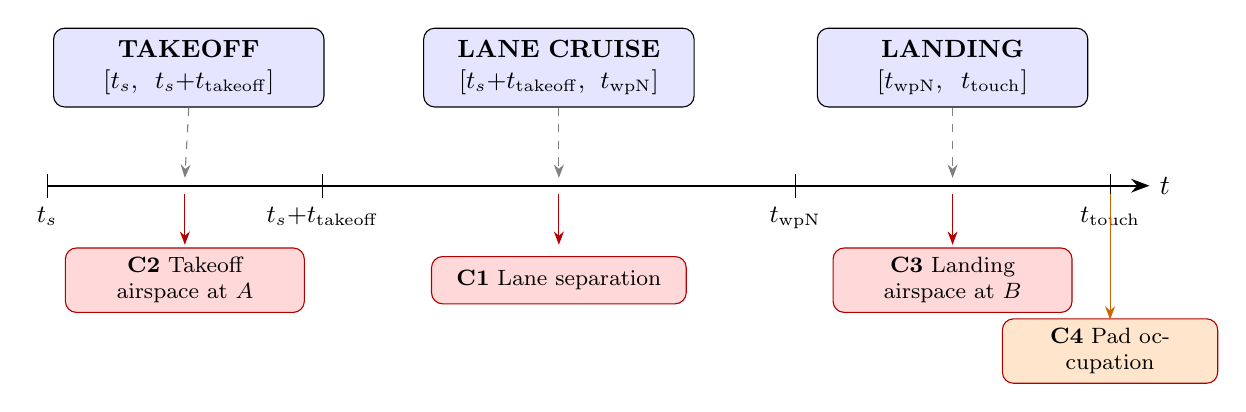
\begin{tikzpicture}[
    >=Stealth,
    timeline/.style={thick},
    phase/.style={draw, rounded corners, fill=blue!10, minimum height=1cm,
                  text width=3.2cm, align=center, font=\small},
    conflict/.style={draw=red!70!black, fill=red!15, rounded corners,
                     minimum height=0.6cm, font=\footnotesize, align=center}
  ]

  % Horizontal timeline
  \draw[timeline,->] (0,0) -- (14,0) node[right]{$t$};

  % Phase boxes
  \node[phase] (takeoff) at (1.8,1.5)
    {\textbf{TAKEOFF}\\\small $[t_s,\;t_s{+}\tto]$};
  \node[phase] (lane) at (6.5,1.5)
    {\textbf{LANE CRUISE}\\\small $[t_s{+}\tto,\;\twpN]$};
  \node[phase] (landing) at (11.5,1.5)
    {\textbf{LANDING}\\\small $[\twpN,\;\ttouch]$};

  % Key time markers on timeline
  \foreach \x/\lbl in {0/$t_s$, 3.5/$t_s{+}\tto$, 9.5/$\twpN$, 13.5/$\ttouch$}
    \draw (\x,0.15) -- (\x,-0.15) node[below]{\small\lbl};

  % Arrows from phases to timeline
  \draw[->,dashed,gray] (takeoff.south) -- (1.75,0.1);
  \draw[->,dashed,gray] (lane.south) -- (6.5,0.1);
  \draw[->,dashed,gray] (landing.south) -- (11.5,0.1);

  % Conflict labels below
  \node[conflict, text width=2.8cm] at (1.75,-1.2)
    {\textbf{C2} Takeoff airspace at~$A$};
  \node[conflict, text width=3.0cm] at (6.5,-1.2)
    {\textbf{C1} Lane separation};
  \node[conflict, text width=2.8cm] at (11.5,-1.2)
    {\textbf{C3} Landing airspace at~$B$};
  \node[conflict, text width=2.5cm, fill=orange!20] at (13.5,-2.1)
    {\textbf{C4} Pad occupation};

  \draw[->,red!70!black] (1.75,-0.1) -- (1.75,-0.75);
  \draw[->,red!70!black] (6.5,-0.1) -- (6.5,-0.75);
  \draw[->,red!70!black] (11.5,-0.1) -- (11.5,-0.75);
  \draw[->,orange!80!black] (13.5,-0.1) -- (13.5,-1.7);

\end{tikzpicture}
\end{center}

\bigskip
\subsection*{6.2\quad Constraint C1 — Minimum Lane Separation}

\paragraph{Setup.}
Consider two drones sharing a lane segment of length $L$.  Let the
\emph{lead} drone (already approved) enter the segment at time $t_j$ with
speed $v_j$, and let the \emph{follower} drone (new request) enter at time
$t_i > t_j$ with speed $v_i$.  Define the time headway
$h = t_i - t_j > 0$.

\paragraph{Spatial gap evolution.}
At time $\tau$ after the follower enters (measuring $\tau = 0$ at follower
entry), the positional gap between follower and lead is:
\begin{equation}
  G(\tau) = v_j h + (v_j - v_i)\tau.
  \label{eq:gap}
\end{equation}
When $v_i > v_j$, the gap decreases.  The minimum gap occurs at the moment
the follower exits the segment, $\tau^* = L / v_i$:
\begin{equation}
  G_{\min} = v_j h - \frac{(v_i - v_j)\,L}{v_i}.
  \label{eq:gmin}
\end{equation}

\paragraph{Safety constraint and minimum headway.}
Safety requires $G_{\min} \ge \MSD + b_j$, where $\MSD$ is the minimum
separation distance and $b_j$ is the body length of the lead drone.
Solving for $h$:
\begin{equation}
  \boxed{
  \hmin(v_i, v_j, L) =
    \frac{\MSD + b_j}{v_j}
    + \frac{\max(0,\, v_i - v_j)\cdot L}{v_i\, v_j}.
  }
  \label{eq:hmin}
\end{equation}
The first term enforces a minimum spatial gap at the segment entry; the second
term compensates for gap closure when the follower is faster.

\paragraph{Applying C1.}
Let $\Delta_s^{\mathrm{new}}$ and $\Delta_s^{\mathrm{appr}}$ denote the elapsed
time from departure to the entry of segment $s$ for the new request and for an
approved plan respectively.  Given a current delay $d$, the follower entry
time is $t_i = t_{\mathrm{des}} + d + \Delta_s^{\mathrm{new}}$ and the lead
entry time is $t_j = t_{\mathrm{appr}} + \Delta_s^{\mathrm{appr}}$.
The follower exit time is $t_i + L/v_i$.

Two safe orderings exist:
\begin{align}
  \text{(new leads):}\quad & t_i + L/v_i + \hmin(v_j, v_i, L) \le t_j,
  \label{eq:new_leads}\\
  \text{(new follows):}\quad & t_i \ge t_j + \hmin(v_i, v_j, L).
  \label{eq:new_follows}
\end{align}
If neither holds, the required delay is derived from \eqref{eq:new_follows}:
\begin{equation}
  d' = t_j + \hmin(v_i, v_j, L) - \Delta_s^{\mathrm{new}} - t_{\mathrm{des}}.
  \label{eq:c1_delay}
\end{equation}
The constraint function is $f_1(d) = \max(d,\; \max_{s\in S} d'_s)$, where
$S$ is the set of lane segments shared with any approved plan.

\bigskip
\subsection*{6.3\quad Constraint C2 — Takeoff Airspace Exclusion}

\paragraph{Airspace window pool.}
For each vertiport $V$, define the \emph{airspace window pool}
$\mathcal{W}(V)$ as the union of:
\begin{itemize}
  \item Takeoff windows $[t_s,\; t_s + \tto]$ of every approved plan departing
    from $V$; and
  \item Descent windows $[\twpN,\; \twpN + \tland]$ of every approved plan
    arriving at $V$.
\end{itemize}
Using a single pool for both ascent and descent operations ensures that an
ascending drone at $V$ and a descending drone at $V$ are automatically
treated as mutually exclusive, without requiring special-case logic.

\paragraph{Advancing past conflicts.}
Define the primitive
\[
  \mathrm{Advance}(t,\, \delta,\, \mathcal{W})
  = \text{smallest } t' \ge t \text{ such that }
    [t', t'+\delta) \cap [s,e) = \emptyset \;\forall\, [s,e)\in\mathcal{W}.
\]
An efficient iterative algorithm for this primitive is:
\begin{algorithm}[H]
\caption{$\mathrm{Advance}(t, \delta, \mathcal{W})$}
\begin{algorithmic}[1]
\For{$k = 1$ \textbf{to} $|\mathcal{W}|+1$}
  \State $\mathcal{C} \gets \{[s,e)\in\mathcal{W} : s < t + \delta \text{ and } e > t\}$
  \If{$\mathcal{C} = \emptyset$} \Return $t$ \EndIf
  \State $t \gets \max\{e : [s,e) \in \mathcal{C}\}$
\EndFor
\end{algorithmic}
\end{algorithm}
\noindent
At each iteration, the window $[t, t+\delta)$ overlaps at least one member of
$\mathcal{C}$.  Advancing to $\max\{e\}$ clears \emph{all} currently
conflicting windows in a single step; hence the loop terminates in at most
$|\mathcal{W}|+1$ steps.

\paragraph{C2 constraint function.}
Given delay $d$, the proposed departure time is $\tdep = t_{\mathrm{des}} + d$.
The constraint function is:
\begin{equation}
  f_2(d) = \mathrm{Advance}(\tdep,\;\tto,\;\mathcal{W}(A)) - t_{\mathrm{des}}.
  \label{eq:c2}
\end{equation}

\bigskip
\subsection*{6.4\quad Constraint C3 — Landing Airspace Exclusion}

The new request's descent begins at $\twpN = t_{\mathrm{des}} + d + \tto + \lane$.
The earliest conflict-free descent start is:
\[
  \twpN^* = \mathrm{Advance}(\twpN,\;\tland,\;\mathcal{W}(B)).
\]
Back-calculating the departure delay corresponding to $\twpN^*$:
\begin{equation}
  f_3(d) = \twpN^* - \tto - \lane - t_{\mathrm{des}}.
  \label{eq:c3}
\end{equation}
The back-calculation step is necessary because $\twpN$ sits at the downstream
end of the flight timeline; any forward shift in $\twpN$ must be translated
into an equivalent upstream shift of the departure delay.

\bigskip
\subsection*{6.5\quad Constraint C4 — Landing Pad Occupancy}

\paragraph{Occupation windows.}
For each approved plan with assigned pad $p$, define an occupation window
$[\ttouch^{\mathrm{appr}},\;\ttouch^{\mathrm{appr}} + \delta_p)$.

\paragraph{Finding the earliest free touchdown.}
For pad $p$, let $\ttouch = t_{\mathrm{des}} + d + \tto + \lane + \tland$.
The earliest free touchdown is found by advancing $\ttouch$ past any
occupation window that \emph{contains} it:
\begin{algorithm}[H]
\caption{Earliest free touchdown on pad $p$}
\begin{algorithmic}[1]
\For{$k = 1$ \textbf{to} $|\mathcal{O}_p|+1$}
  \State $\mathcal{B} \gets \{[s,e)\in\mathcal{O}_p : s \le \ttouch < e\}$
  \If{$\mathcal{B} = \emptyset$} \textbf{break} \EndIf
  \State $\ttouch \gets \min\{e : [s,e) \in \mathcal{B}\}$
\EndFor
\end{algorithmic}
\end{algorithm}
\noindent
Note the use of $\min\{e\}$ rather than $\max\{e\}$: a touchdown is a
\emph{point event}, so only the single window enclosing the point must be
cleared; no duration needs to fit between windows.

\paragraph{C4 constraint function.}
For each pad $p$ at vertiport $B$, compute the corresponding departure delay:
\begin{equation}
  d_p = \ttouch^*_p - \tland - \lane - \tto - t_{\mathrm{des}}.
  \label{eq:c4}
\end{equation}
Select the pad $p^*$ minimising $d_p$, and set $f_4(d) = d_{p^*}$.

\bigskip
\subsection*{6.6\quad Fixed-Point Iteration and Convergence}

\paragraph{Composed constraint map.}
Define the composed constraint map:
\begin{equation}
  F(d) = f_4\bigl(f_3\bigl(f_2\bigl(f_1(d)\bigr)\bigr)\bigr).
  \label{eq:F}
\end{equation}

\begin{theorem}[Existence and convergence of minimum feasible delay]
\label{thm:convergence}
Each function $f_k$ is monotone non-decreasing and bounded above by
$T_{\max} = \max\{e : [s,e)\in \bigcup_k \mathcal{W}_k\}$.  Consequently:
\begin{enumerate}[label=(\roman*)]
  \item $F$ is monotone non-decreasing and bounded above by $T_{\max}$.
  \item By the Knaster--Tarski theorem, $F$ has a least fixed point
    $d^* = \min\{d \ge 0 : F(d) = d\}$.
  \item The orbit $d_0 = 0,\; d_{k+1} = F(d_k)$ is non-decreasing and
    converges to $d^*$ in at most $N$ steps, where $N$ is the total number
    of distinct window endpoints across all constraints.
\end{enumerate}
\end{theorem}

\begin{proof}[Proof sketch]
Monotonicity of $f_1$: increasing $d$ advances all follower entry times,
which can only widen headways, never create new mandatory delays beyond those
already enforced by \eqref{eq:c1_delay}; the maximum of monotone functions
is monotone.  Monotonicity of $f_2$, $f_3$ follows directly from the
monotonicity of the \textsc{Advance} primitive: if $t$ increases, the
returned $t' \ge t$ cannot decrease.  Monotonicity of $f_4$ follows
similarly.  Composition preserves monotonicity.  Boundedness: the
\textsc{Advance} primitive returns a value no greater than the latest window
endpoint in the pool, which is finite; back-calculations preserve
boundedness.  The Knaster--Tarski theorem then guarantees a least fixed
point, and the orbit from the bottom element $d_0 = 0$ is non-decreasing
and bounded, hence convergent.
\end{proof}

\paragraph{Algorithm — single request.}

\begin{algorithm}[H]
\caption{Single-Request Conflict Resolution}
\label{alg:single}
\begin{algorithmic}[1]
\Require Flight-plan request $r$, approved-plan set $\mathcal{A}$, tolerance
  $\varepsilon = 0.01$~s, max iterations $K = 100$
\Ensure \texttt{ResolveResult}
\State $d \gets 0$
\For{$k = 1$ \textbf{to} $K$}
  \State $d_{\mathrm{prev}} \gets d$
  \State $d \gets f_1(d,\,r,\,\mathcal{A})$ \Comment{Lane separation (C1)}
  \State $d \gets f_2(d,\,r,\,\mathcal{A})$ \Comment{Takeoff airspace (C2)}
  \State $d \gets f_3(d,\,r,\,\mathcal{A})$ \Comment{Landing airspace (C3)}
  \State $(d,\, p^*) \gets f_4(d,\,r,\,\mathcal{A})$ \Comment{Pad occupancy (C4)}
  \If{$|d - d_{\mathrm{prev}}| < \varepsilon$} \textbf{break} \EndIf
\EndFor
\If{$d \le r.\texttt{max\_wait\_time}$}
  \Return $\texttt{APPROVED}$, $t_{\mathrm{des}} + d$, $d$, $p^*$
\Else
  \Return $\texttt{REJECTED}$, reason
\EndIf
\end{algorithmic}
\end{algorithm}

\paragraph{Convergence in practice.}
Because the number of distinct window endpoints is bounded by twice the number
of approved plans, and in typical UAM scenarios the number of active plans
within a time horizon is small, Algorithm~\ref{alg:single} converges within
2--4 iterations in normal operation.

\paragraph{Cascade example.}
The following scenario illustrates three-round convergence:

\begin{itemize}
  \item Plans $P_1, P_2, P_3$ depart from vertiport $A$ at $t=0, 10, 20$\,s,
    blocking airspace $A$ until $t=30$\,s.
  \item Plan $P_5$ touches down at $B$ at $t=34$\,s; pad $B_1$ busy on
    $[34, 94)$\,s.
  \item Plan $P_6$ touches down at $B$ at $t=94$\,s; pad $B_1$ busy on
    $[94, 154)$\,s.
  \item Plan $P_7$ departs $A$ at $t=130$\,s on the same lane as the new
    request, occupying airspace $A$ on $[130, 140)$\,s.
\end{itemize}

\noindent\textit{Round 1:}
$f_2$: $\tdep = 0$ conflicts with $P_1,P_2,P_3$ $\Rightarrow$
$d = 30$\,s.
$f_4$: $\ttouch = 54$ lies in $[34,94)$ $\Rightarrow$ jump to 94, lies in
$[94,154)$ $\Rightarrow$ jump to 154; required start $= 130$ $\Rightarrow$
$d = 130$\,s.

\noindent\textit{Round 2:}
$f_1$: follower entry $= 140 = P_7$'s entry; conflict $\Rightarrow$
$d = 131$\,s.
$f_2$: window $[131,141)$ overlaps $P_7$'s $[130,140)$ $\Rightarrow$
advance to 140; $d = 140$\,s.

\noindent\textit{Round 3:}
$f_1$: follower entry $= 150 > 141 = t_j + \hmin$ $\Rightarrow$ safe.
$f_2$: $[140,150)$ does not overlap $[130,140)$ $\Rightarrow$ safe.
$f_3, f_4$: unchanged.
$|d - d_{\mathrm{prev}}| = 0 < \varepsilon$ $\Rightarrow$ \textbf{converged}
at $d^* = 140$\,s.

\bigskip
\subsection*{6.7\quad Batch Resolution with Priority Ordering}

When multiple requests arrive simultaneously, resolving them on a common
static pool can produce post-approval conflicts (e.g., two requests may both
be assigned the same pad at the same time before either is committed to the
pool).  The disclosed batch procedure avoids this:

\begin{algorithm}[H]
\caption{Priority-Based Batch Resolution}
\label{alg:batch}
\begin{algorithmic}[1]
\Require Requests $\{r_1, \ldots, r_m\}$ with priorities $\{p_1,\ldots,p_m\}$,
  initial approved set $\mathcal{A}$
\Ensure Per-request \texttt{ResolveResult} in original order
\State $\sigma \gets \mathrm{argsort}(\text{priority ASC, desired\_start ASC})$
\State $\mathcal{A}' \gets \mathcal{A}$
\For{$i \in \sigma$}
  \State $\mathrm{result}[i] \gets \mathrm{Resolve}(r_i, \mathcal{A}')$
  \If{$\mathrm{result}[i].\texttt{approved}$}
    \State $\mathcal{A}' \gets \mathcal{A}' \cup
           \{\mathrm{ApprovedPlan}(\mathrm{result}[i])\}$
  \EndIf
\EndFor
\Return $\mathrm{result}[\text{original order}]$
\end{algorithmic}
\end{algorithm}

\noindent
By augmenting $\mathcal{A}'$ after each approval, higher-priority requests
effectively ``lock'' resources before lower-priority requests are evaluated,
guaranteeing conflict-free results across the entire batch.

\bigskip
\subsection*{6.8\quad System Architecture}

The disclosed system comprises:

\begin{enumerate}[label=(\Alph*)]
  \item A \textbf{Flight Plan Store} maintaining the set $\mathcal{A}$ of
    currently approved flight plans, with indexed lookup by vertiport
    identifier and time range.

  \item A \textbf{Constraint Engine} implementing $f_1, f_2, f_3, f_4$ and
    the \textsc{Advance} primitive.

  \item A \textbf{Resolver} orchestrating the fixed-point iteration
    (Algorithm~\ref{alg:single}) and batch resolution
    (Algorithm~\ref{alg:batch}).

  \item A \textbf{Communication Interface} accepting flight-plan requests via
    a RESTful API or message queue and returning structured
    \texttt{ResolveResult} objects.
\end{enumerate}

The system may be deployed as a microservice on commodity cloud infrastructure,
as a process on a UAM network management server, or as firmware on a
ground-based vertiport controller.

% =============================================================================
\section{Claims}
% =============================================================================

\begin{claim}
A computer-implemented method for resolving scheduling conflicts in a Urban Air
Mobility (UAM) network, the method comprising:
\begin{enumerate}[label=\alph*)]
  \item receiving a flight-plan request comprising a departure vertiport
    identifier, a destination vertiport identifier, a sequence of waypoints, a
    sequence of per-segment cruise speeds, a vertical ascent duration, a
    vertical descent duration, a desired departure time, and a maximum wait
    time;
  \item accessing a set of previously approved flight plans stored in a flight
    plan store;
  \item iteratively applying, until convergence, a composed constraint map
    $F = f_4 \circ f_3 \circ f_2 \circ f_1$ to an initial departure delay of
    zero, wherein each $f_k$ is a monotone non-decreasing function that maps a
    current departure delay to a departure delay satisfying constraint $C_k$;
  \item determining that the flight-plan request is approved when the converged
    delay does not exceed the maximum wait time; and
  \item determining that the flight-plan request is rejected when the converged
    delay exceeds the maximum wait time.
\end{enumerate}
\end{claim}

\begin{claim}
The method of claim~1, wherein constraint $C_1$ enforces a minimum spatial
separation between the new flight plan and each approved flight plan sharing at
least one lane segment, wherein the minimum time headway is computed as:
\[
  \hmin(v_i, v_j, L) =
    \frac{\MSD + b_j}{v_j}
    + \frac{\max(0,\, v_i - v_j)\cdot L}{v_i\, v_j},
\]
where $v_i$ is the follower cruise speed, $v_j$ is the lead cruise speed, $L$
is the segment length, $\MSD$ is a minimum separation distance, and $b_j$ is
the body length of the lead vehicle.
\end{claim}

\begin{claim}
The method of claim~1, wherein constraint $C_2$ enforces mutual exclusion of a
vertical takeoff corridor above the departure vertiport by applying the
\textsc{Advance} primitive to find the earliest departure time $\tdep^*$ such
that the interval $[\tdep^*, \tdep^* + \tto)$ does not overlap any window in
a pool comprising all approved takeoff and landing airspace windows at the
departure vertiport.
\end{claim}

\begin{claim}
The method of claim~1, wherein constraint $C_3$ enforces mutual exclusion of a
vertical landing corridor above the destination vertiport by:
\begin{enumerate}[label=\alph*)]
  \item computing the arrival waypoint time $\twpN$ from the current departure
    delay;
  \item applying the \textsc{Advance} primitive to find the earliest conflict-free
    $\twpN^*$; and
  \item back-calculating the required departure delay as
    $d' = \twpN^* - \tto - \lane - t_{\mathrm{des}}$.
\end{enumerate}
\end{claim}

\begin{claim}
The method of claim~1, wherein constraint $C_4$ enforces pad-occupancy
exclusion by:
\begin{enumerate}[label=\alph*)]
  \item for each available landing pad at the destination vertiport, computing
    the earliest touchdown time $\ttouch^*$ not falling within any pad
    occupation window by advancing $\ttouch$ to the end of each enclosing
    window;
  \item computing a pad-specific departure delay
    $d_p = \ttouch^* - \tland - \lane - \tto - t_{\mathrm{des}}$ for each
    pad $p$; and
  \item selecting the pad yielding the minimum $d_p$ and returning that delay.
\end{enumerate}
\end{claim}

\begin{claim}
The method of claim~3, wherein the pool of airspace windows at any vertiport
comprises both the takeoff windows of flights departing from that vertiport and
the descent windows of flights arriving at that vertiport, thereby enforcing
mutual exclusion between ascending and descending vehicles in a single unified
pool without dedicated special-case logic.
\end{claim}

\begin{claim}
The method of claim~1, wherein the composed constraint map $F$ is guaranteed to
converge to a least fixed point $d^*$ by virtue of the monotonicity and
boundedness of each $f_k$, as established by the Knaster--Tarski fixed-point
theorem applied to the complete lattice $([0, T_{\max}], \le)$ where $T_{\max}$
is the maximum window endpoint across all constraint pools.
\end{claim}

\begin{claim}
The method of claim~1, further comprising resolving a batch of simultaneous
flight-plan requests by:
\begin{enumerate}[label=\alph*)]
  \item sorting the requests by ascending priority value and, within equal
    priorities, by ascending desired departure time;
  \item processing each request in sorted order using the method of claim~1
    against an augmented approved-plan set; and
  \item after each approval, adding the newly approved plan to the augmented
    approved-plan set before processing the next request.
\end{enumerate}
\end{claim}

\begin{claim}
The method of claim~1, wherein the \textsc{Advance} primitive
$\mathrm{Advance}(t, \delta, \mathcal{W})$ finds the smallest $t' \ge t$ such
that $[t', t'+\delta)$ is disjoint from every window in $\mathcal{W}$ by
iteratively setting $t$ to the maximum endpoint among all windows overlapping
$[t, t+\delta)$, terminating in at most $|\mathcal{W}|+1$ iterations.
\end{claim}

\begin{claim}
A non-transitory computer-readable medium storing instructions that, when
executed by one or more processors, implement the method of any one of
claims~1--9.
\end{claim}

\begin{claim}
A system for conflict-free flight-plan scheduling in a UAM network, the system
comprising:
\begin{enumerate}[label=\alph*)]
  \item a flight plan store configured to maintain a set of approved flight
    plans indexed by vertiport identifier and time range;
  \item a constraint engine implementing functions $f_1, f_2, f_3, f_4$ each
    mapping a departure delay to a constraint-satisfying departure delay; and
  \item a resolver coupled to the flight plan store and the constraint engine,
    configured to execute the fixed-point iteration of Algorithm~1 and the
    priority-based batch procedure of Algorithm~2; and
  \item a communication interface configured to receive flight-plan requests and
    return structured resolution results.
\end{enumerate}
\end{claim}

% =============================================================================
\section{Abstract of the Disclosure}
% =============================================================================

A conflict-resolution system for UAM flight plans enforces four physical safety
constraints — (C1)~lane separation, (C2)~takeoff airspace exclusion,
(C3)~landing airspace exclusion, (C4)~pad occupancy — each formulated as a
monotone non-decreasing delay function.  Iterating the composed constraint map
$F = f_4 \circ f_3 \circ f_2 \circ f_1$ from delay zero converges, by the
Knaster--Tarski theorem, to the minimum feasible departure delay in a finite
number of steps (typically 2--4 in practice).  A priority-based sequential
batch procedure handles simultaneous requests without post-approval conflicts.

% =============================================================================

\end{document}
